%%%% Paramétrage du TD %%%%
\def\xxactivite{Révisions \ifprof -- Corrigé \else \fi} % \normalsize \vspace{-.4cm}
\def\xxauteur{\textsl{Xavier Pessoles}}


\def\xxnumchapitre{Révision 1 \vspace{.2cm}}
\def\xxchapitre{\hspace{.12cm} Résolution des problèmes de statique -- Statique 3D}
\def\xxonglet{\textsf{Rév -- Stat}}
\def\xxactivite{TD 01}
\def\xxauteur{\textsl{Xavier Pessoles}}

\def\xxpied{%
Révision statique -- Résolution des problèmes de statique 3D\\
Fiche 1 -- \xxactivite%
}

\def\xxtitreexo{Micromanipulateur compact pour la chirurgie endoscopique ($\text{MC}^2\text{E}$)}
\def\xxsourceexo{\hspace{.2cm} \footnotesize{Concours Commun Mines Ponts 2016}}

\def\xxcompetences{%
\textsl{%
\textbf{Savoirs et compétences :}\\} \vspace{-.5cm}
\begin{itemize}
\item \textit{Res2.C18} : principe fondamental de la statique;
\item \textit{Res2.C19} : équilibre d’un solide, d’un ensemble de solides;
\item \textit{Res2.C20} : théorème des actions réciproques.
\end{itemize}
}

\def\xxauteur{\textsl{Xavier Pessoles}}


\def\xxfigures{
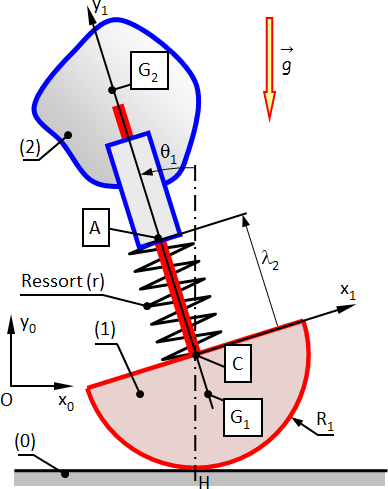
\includegraphics[width=.55\textwidth]{fig_01}
}%figues de la page de garde


\iflivret
\pagestyle{empty}


%%%%%%%% PAGE DE GARDE COURS
\ifcours
% ==== BANDEAU DES TITRES ==== 
\begin{tikzpicture}[remember picture,overlay]
\node at (current page.north west)
{\begin{tikzpicture}[remember picture,overlay]
\node[anchor=north west,inner sep=0pt] at (0,0) {\includegraphics[width=\paperwidth]{\thechapterimage}};
\draw[anchor=west] (-2cm,-8cm) node [line width=2pt,rounded corners=15pt,draw=ocre,fill=white,fill opacity=0.6,inner sep=40pt]{\strut\makebox[22cm]{}};
\draw[anchor=west] (1cm,-8cm) node {\huge\sffamily\bfseries\color{black} %
\begin{minipage}{1cm}
\rotatebox{90}{\LARGE\sffamily\textsc{\color{ocre}\textbf{\xxnumpartie}}}
\end{minipage} \hfill
\begin{minipage}[c]{14cm}
\begin{titrepartie}
\begin{flushright}
\renewcommand{\baselinestretch}{1.1} 
\Large\sffamily\textsc{\textbf{\xxpartie}}
\renewcommand{\baselinestretch}{1} 
\end{flushright}
\end{titrepartie}
\end{minipage} \hfill
\begin{minipage}[c]{3.5cm}
{\large\sffamily\textsc{\textbf{\color{ocre} \discipline}}}
\end{minipage} 
 };
\end{tikzpicture}};
\end{tikzpicture}
% ==== FIN BANDEAU DES TITRES ==== 


% ==== ONGLET 
\begin{tikzpicture}[overlay]
\node[shape=rectangle, 
      rounded corners = .25 cm,
	  draw= ocre,
	  line width=2pt, 
	  fill = ocre!10,
	  minimum width  = 2.5cm,
	  minimum height = 3cm,] at (18.3cm,0) {};
\node at (17.7cm,0) {\rotatebox{90}{\textbf{\Large\color{ocre}{\classe}}}};
%{};
\end{tikzpicture}
% ==== FIN ONGLET 


\vspace{3.5cm}

\begin{tikzpicture}[remember picture,overlay]
\draw[anchor=west] (-2cm,-6cm) node {\huge\sffamily\bfseries\color{black} %
\begin{minipage}{2cm}
\begin{center}
\LARGE\sffamily\textsc{\color{ocre}\textbf{\xxactivite}}
\end{center}
\end{minipage} \hfill
\begin{minipage}[c]{15cm}
\begin{titrechapitre}
\renewcommand{\baselinestretch}{1.1} 
\Large\sffamily\textsc{\textbf{\xxnumchapitre}}

\Large\sffamily\textsc{\textbf{\xxchapitre}}
\vspace{.5cm}

\renewcommand{\baselinestretch}{1} 
\normalsize\normalfont
\xxcompetences
\end{titrechapitre}
\end{minipage}  };
\end{tikzpicture}
\vfill

\begin{flushright}
\begin{minipage}[c]{.3\linewidth}
\begin{center}
\xxfigures
\end{center}
\end{minipage}\hfill
\begin{minipage}[c]{.6\linewidth}
\startcontents
%\printcontents{}{1}{}
\printcontents{}{1}{}
\end{minipage}
\end{flushright}

\begin{tikzpicture}[remember picture,overlay]
\draw[anchor=west] (4.5cm,-.7cm) node {
\begin{minipage}[c]{.2\linewidth}
\begin{flushright}

\includegraphics[width=2cm]{logoCC}
\end{flushright}
\end{minipage}
\begin{minipage}[c]{.2\linewidth}
\textsl{\xxauteur} \\
\textsl{\classe}
\end{minipage}
 };
\end{tikzpicture}

\newpage
\pagestyle{fancy}

%\newpage
%\pagestyle{fancy}

\else
\fi
%% FIN PAGE DE GARDE DES COURS

%%%%%%%% PAGE DE GARDE TD
\iftd
%\begin{tikzpicture}[remember picture,overlay]
%\node at (current page.north west)
%{\begin{tikzpicture}[remember picture,overlay]
%\draw[anchor=west] (-2cm,-3.25cm) node [line width=2pt,rounded corners=15pt,draw=ocre,fill=white,fill opacity=0.6,inner sep=40pt]{\strut\makebox[22cm]{}};
%\draw[anchor=west] (1cm,-3.25cm) node {\huge\sffamily\bfseries\color{black} %
%\begin{minipage}{1cm}
%\rotatebox{90}{\LARGE\sffamily\textsc{\color{ocre}\textbf{\xxnumpartie}}}
%\end{minipage} \hfill
%\begin{minipage}[c]{13.5cm}
%\begin{titrepartie}
%\begin{flushright}
%\renewcommand{\baselinestretch}{1.1} 
%\Large\sffamily\textsc{\textbf{\xxpartie}}
%\renewcommand{\baselinestretch}{1} 
%\end{flushright}
%\end{titrepartie}
%\end{minipage} \hfill
%\begin{minipage}[c]{3.5cm}
%{\large\sffamily\textsc{\textbf{\color{ocre} \discipline}}}
%\end{minipage} 
% };
%\end{tikzpicture}};
%\end{tikzpicture}

%%%%%%%%%% PAGE DE GARDE TD %%%%%%%%%%%%%%%
%\begin{tikzpicture}[overlay]
%\node[shape=rectangle, 
%      rounded corners = .25 cm,
%	  draw= ocre,
%	  line width=2pt, 
%	  fill = ocre!10,
%	  minimum width  = 2.5cm,
%	  minimum height = 2.5cm,] at (18.5cm,0) {};
%\node at (17.7cm,0) {\rotatebox{90}{\textbf{\Large\color{ocre}{\classe}}}};
%%{};
%\end{tikzpicture}

% PARTIE ET CHAPITRE
%\begin{tikzpicture}[remember picture,overlay]
%\draw[anchor=west] (-1cm,-2.1cm) node {\large\sffamily\bfseries\color{black} %
%\begin{minipage}[c]{15cm}
%\begin{flushleft}
%\xxnumchapitre \\
%\xxchapitre
%\end{flushleft}
%\end{minipage}  };
%\end{tikzpicture}

% BANDEAU EXO
\iflivret % SI LIVRET
\begin{tikzpicture}[remember picture,overlay]
\draw[anchor=west] (-2cm,-3.3cm) node {\huge\sffamily\bfseries\color{black} %
\begin{minipage}{5cm}
\begin{center}
\LARGE\sffamily\color{ocre}\textbf{\textsc{\xxactivite}}

\begin{center}
\xxfigures
\end{center}

\end{center}
\end{minipage} \hfill
\begin{minipage}[c]{12cm}
\begin{titrechapitre}
\renewcommand{\baselinestretch}{1.1} 
\large\sffamily\textbf{\textsc{\xxtitreexo}}

\small\sffamily{\textbf{\textit{\color{black!70}\xxsourceexo}}}
\vspace{.5cm}

\renewcommand{\baselinestretch}{1} 
\normalsize\normalfont
\xxcompetences
\end{titrechapitre}
\end{minipage}};
\end{tikzpicture}
\else % ELSE NOT LIVRET
\begin{tikzpicture}[remember picture,overlay]
\draw[anchor=west] (-2cm,-4.5cm) node {\huge\sffamily\bfseries\color{black} %
\begin{minipage}{5cm}
\begin{center}
\LARGE\sffamily\color{ocre}\textbf{\textsc{\xxactivite}}

\begin{center}
\xxfigures
\end{center}

\end{center}
\end{minipage} \hfill
\begin{minipage}[c]{12cm}
\begin{titrechapitre}
\renewcommand{\baselinestretch}{1.1} 
\large\sffamily\textbf{\textsc{\xxtitreexo}}

\small\sffamily{\textbf{\textit{\color{black!70}\xxsourceexo}}}
\vspace{.5cm}

\renewcommand{\baselinestretch}{1} 
\normalsize\normalfont
\xxcompetences
\end{titrechapitre}
\end{minipage}};
\end{tikzpicture}

\fi

\else   % FIN IF TD
\fi


%%%%%%%% PAGE DE GARDE FICHE
\iffiche
\begin{tikzpicture}[remember picture,overlay]
\node at (current page.north west)
{\begin{tikzpicture}[remember picture,overlay]
\draw[anchor=west] (-2cm,-2.25cm) node [line width=2pt,rounded corners=15pt,draw=ocre,fill=white,fill opacity=0.6,inner sep=40pt]{\strut\makebox[22cm]{}};
\draw[anchor=west] (1cm,-2.25cm) node {\huge\sffamily\bfseries\color{black} %
\begin{minipage}{1cm}
\rotatebox{90}{\LARGE\sffamily\textsc{\color{ocre}\textbf{\xxnumpartie}}}
\end{minipage} \hfill
\begin{minipage}[c]{14cm}
\begin{titrepartie}
\begin{flushright}
\renewcommand{\baselinestretch}{1.1} 
\large\sffamily\textsc{\textbf{\xxpartie} \\} 

\vspace{.2cm}

\normalsize\sffamily\textsc{\textbf{\xxnumchapitre -- \xxchapitre}}
\renewcommand{\baselinestretch}{1} 
\end{flushright}
\end{titrepartie}
\end{minipage} \hfill
\begin{minipage}[c]{3.5cm}
{\large\sffamily\textsc{\textbf{\color{ocre} \discipline}}}
\end{minipage} 
 };
\end{tikzpicture}};
\end{tikzpicture}

\iflivret
\begin{tikzpicture}[overlay]
\node[shape=rectangle, 
      rounded corners = .25 cm,
	  draw= ocre,
	  line width=2pt, 
	  fill = ocre!10,
	  minimum width  = 2.5cm,
	  minimum height = 2.5cm,] at (18.5cm,.5cm) {};
\node at (17.9cm,.5cm) {\rotatebox{90}{\textsf{\textbf{\large\color{ocre}{\classe}}}}};
%{};
\end{tikzpicture}
\else
\begin{tikzpicture}[overlay]
\node[shape=rectangle, 
      rounded corners = .25 cm,
	  draw= ocre,
	  line width=2pt, 
	  fill = ocre!10,
	  minimum width  = 2.5cm,
%	  minimum height = 2.5cm,] at (18.5cm,1.1cm) {};
	  minimum height = 2.5cm,] at (18.6cm,0.5cm) {};
\node at (18cm,0.5cm) {\rotatebox{90}{\textsf{\textbf{\large\color{ocre}{\classe}}}}};
%{};
\end{tikzpicture}

\fi

\else
\fi



\else
\pagestyle{empty}


%%%%%%%% PAGE DE GARDE COURS
\ifcours
% ==== BANDEAU DES TITRES ==== 
\begin{tikzpicture}[remember picture,overlay]
\node at (current page.north west)
{\begin{tikzpicture}[remember picture,overlay]
\node[anchor=north west,inner sep=0pt] at (0,0) {\includegraphics[width=\paperwidth]{\thechapterimage}};
\draw[anchor=west] (-2cm,-8cm) node [line width=2pt,rounded corners=15pt,draw=ocre,fill=white,fill opacity=0.6,inner sep=40pt]{\strut\makebox[22cm]{}};
\draw[anchor=west] (1cm,-8cm) node {\huge\sffamily\bfseries\color{black} %
\begin{minipage}{1cm}
\rotatebox{90}{\LARGE\sffamily\textsc{\color{ocre}\textbf{\xxnumpartie}}}
\end{minipage} \hfill
\begin{minipage}[c]{14cm}
\begin{titrepartie}
\begin{flushright}
\renewcommand{\baselinestretch}{1.1} 
\Large\sffamily\textsc{\textbf{\xxpartie}}
\renewcommand{\baselinestretch}{1} 
\end{flushright}
\end{titrepartie}
\end{minipage} \hfill
\begin{minipage}[c]{3.5cm}
{\large\sffamily\textsc{\textbf{\color{ocre} \discipline}}}
\end{minipage} 
 };
\end{tikzpicture}};
\end{tikzpicture}
% ==== FIN BANDEAU DES TITRES ==== 


% ==== ONGLET 
\begin{tikzpicture}[overlay]
\node[shape=rectangle, 
      rounded corners = .25 cm,
	  draw= ocre,
	  line width=2pt, 
	  fill = ocre!10,
	  minimum width  = 2.5cm,
	  minimum height = 3cm,] at (18.3cm,0) {};
\node at (17.7cm,0) {\rotatebox{90}{\textbf{\Large\color{ocre}{\classe}}}};
%{};
\end{tikzpicture}
% ==== FIN ONGLET 


\vspace{3.5cm}

\begin{tikzpicture}[remember picture,overlay]
\draw[anchor=west] (-2cm,-6cm) node {\huge\sffamily\bfseries\color{black} %
\begin{minipage}{2cm}
\begin{center}
\LARGE\sffamily\textsc{\color{ocre}\textbf{\xxactivite}}
\end{center}
\end{minipage} \hfill
\begin{minipage}[c]{15cm}
\begin{titrechapitre}
\renewcommand{\baselinestretch}{1.1} 
\Large\sffamily\textsc{\textbf{\xxnumchapitre}}

\Large\sffamily\textsc{\textbf{\xxchapitre}}
\vspace{.5cm}

\renewcommand{\baselinestretch}{1} 
\normalsize\normalfont
\xxcompetences
\end{titrechapitre}
\end{minipage}  };
\end{tikzpicture}
\vfill

\begin{flushright}
\begin{minipage}[c]{.3\linewidth}
\begin{center}
\xxfigures
\end{center}
\end{minipage}\hfill
\begin{minipage}[c]{.6\linewidth}
\startcontents
%\printcontents{}{1}{}
\printcontents{}{1}{}
\end{minipage}
\end{flushright}

\begin{tikzpicture}[remember picture,overlay]
\draw[anchor=west] (4.5cm,-.7cm) node {
\begin{minipage}[c]{.2\linewidth}
\begin{flushright}

\includegraphics[width=2cm]{logoCC}
\end{flushright}
\end{minipage}
\begin{minipage}[c]{.2\linewidth}
\textsl{\xxauteur} \\
\textsl{\classe}
\end{minipage}
 };
\end{tikzpicture}

\newpage
\pagestyle{fancy}

%\newpage
%\pagestyle{fancy}

\else
\fi
%% FIN PAGE DE GARDE DES COURS

%%%%%%%% PAGE DE GARDE TD
\iftd
%\begin{tikzpicture}[remember picture,overlay]
%\node at (current page.north west)
%{\begin{tikzpicture}[remember picture,overlay]
%\draw[anchor=west] (-2cm,-3.25cm) node [line width=2pt,rounded corners=15pt,draw=ocre,fill=white,fill opacity=0.6,inner sep=40pt]{\strut\makebox[22cm]{}};
%\draw[anchor=west] (1cm,-3.25cm) node {\huge\sffamily\bfseries\color{black} %
%\begin{minipage}{1cm}
%\rotatebox{90}{\LARGE\sffamily\textsc{\color{ocre}\textbf{\xxnumpartie}}}
%\end{minipage} \hfill
%\begin{minipage}[c]{13.5cm}
%\begin{titrepartie}
%\begin{flushright}
%\renewcommand{\baselinestretch}{1.1} 
%\Large\sffamily\textsc{\textbf{\xxpartie}}
%\renewcommand{\baselinestretch}{1} 
%\end{flushright}
%\end{titrepartie}
%\end{minipage} \hfill
%\begin{minipage}[c]{3.5cm}
%{\large\sffamily\textsc{\textbf{\color{ocre} \discipline}}}
%\end{minipage} 
% };
%\end{tikzpicture}};
%\end{tikzpicture}

%%%%%%%%%% PAGE DE GARDE TD %%%%%%%%%%%%%%%
%\begin{tikzpicture}[overlay]
%\node[shape=rectangle, 
%      rounded corners = .25 cm,
%	  draw= ocre,
%	  line width=2pt, 
%	  fill = ocre!10,
%	  minimum width  = 2.5cm,
%	  minimum height = 2.5cm,] at (18.5cm,0) {};
%\node at (17.7cm,0) {\rotatebox{90}{\textbf{\Large\color{ocre}{\classe}}}};
%%{};
%\end{tikzpicture}

% PARTIE ET CHAPITRE
%\begin{tikzpicture}[remember picture,overlay]
%\draw[anchor=west] (-1cm,-2.1cm) node {\large\sffamily\bfseries\color{black} %
%\begin{minipage}[c]{15cm}
%\begin{flushleft}
%\xxnumchapitre \\
%\xxchapitre
%\end{flushleft}
%\end{minipage}  };
%\end{tikzpicture}

% BANDEAU EXO
\iflivret % SI LIVRET
\begin{tikzpicture}[remember picture,overlay]
\draw[anchor=west] (-2cm,-3.3cm) node {\huge\sffamily\bfseries\color{black} %
\begin{minipage}{5cm}
\begin{center}
\LARGE\sffamily\color{ocre}\textbf{\textsc{\xxactivite}}

\begin{center}
\xxfigures
\end{center}

\end{center}
\end{minipage} \hfill
\begin{minipage}[c]{12cm}
\begin{titrechapitre}
\renewcommand{\baselinestretch}{1.1} 
\large\sffamily\textbf{\textsc{\xxtitreexo}}

\small\sffamily{\textbf{\textit{\color{black!70}\xxsourceexo}}}
\vspace{.5cm}

\renewcommand{\baselinestretch}{1} 
\normalsize\normalfont
\xxcompetences
\end{titrechapitre}
\end{minipage}};
\end{tikzpicture}
\else % ELSE NOT LIVRET
\begin{tikzpicture}[remember picture,overlay]
\draw[anchor=west] (-2cm,-4.5cm) node {\huge\sffamily\bfseries\color{black} %
\begin{minipage}{5cm}
\begin{center}
\LARGE\sffamily\color{ocre}\textbf{\textsc{\xxactivite}}

\begin{center}
\xxfigures
\end{center}

\end{center}
\end{minipage} \hfill
\begin{minipage}[c]{12cm}
\begin{titrechapitre}
\renewcommand{\baselinestretch}{1.1} 
\large\sffamily\textbf{\textsc{\xxtitreexo}}

\small\sffamily{\textbf{\textit{\color{black!70}\xxsourceexo}}}
\vspace{.5cm}

\renewcommand{\baselinestretch}{1} 
\normalsize\normalfont
\xxcompetences
\end{titrechapitre}
\end{minipage}};
\end{tikzpicture}

\fi

\else   % FIN IF TD
\fi


%%%%%%%% PAGE DE GARDE FICHE
\iffiche
\begin{tikzpicture}[remember picture,overlay]
\node at (current page.north west)
{\begin{tikzpicture}[remember picture,overlay]
\draw[anchor=west] (-2cm,-2.25cm) node [line width=2pt,rounded corners=15pt,draw=ocre,fill=white,fill opacity=0.6,inner sep=40pt]{\strut\makebox[22cm]{}};
\draw[anchor=west] (1cm,-2.25cm) node {\huge\sffamily\bfseries\color{black} %
\begin{minipage}{1cm}
\rotatebox{90}{\LARGE\sffamily\textsc{\color{ocre}\textbf{\xxnumpartie}}}
\end{minipage} \hfill
\begin{minipage}[c]{14cm}
\begin{titrepartie}
\begin{flushright}
\renewcommand{\baselinestretch}{1.1} 
\large\sffamily\textsc{\textbf{\xxpartie} \\} 

\vspace{.2cm}

\normalsize\sffamily\textsc{\textbf{\xxnumchapitre -- \xxchapitre}}
\renewcommand{\baselinestretch}{1} 
\end{flushright}
\end{titrepartie}
\end{minipage} \hfill
\begin{minipage}[c]{3.5cm}
{\large\sffamily\textsc{\textbf{\color{ocre} \discipline}}}
\end{minipage} 
 };
\end{tikzpicture}};
\end{tikzpicture}

\iflivret
\begin{tikzpicture}[overlay]
\node[shape=rectangle, 
      rounded corners = .25 cm,
	  draw= ocre,
	  line width=2pt, 
	  fill = ocre!10,
	  minimum width  = 2.5cm,
	  minimum height = 2.5cm,] at (18.5cm,.5cm) {};
\node at (17.9cm,.5cm) {\rotatebox{90}{\textsf{\textbf{\large\color{ocre}{\classe}}}}};
%{};
\end{tikzpicture}
\else
\begin{tikzpicture}[overlay]
\node[shape=rectangle, 
      rounded corners = .25 cm,
	  draw= ocre,
	  line width=2pt, 
	  fill = ocre!10,
	  minimum width  = 2.5cm,
%	  minimum height = 2.5cm,] at (18.5cm,1.1cm) {};
	  minimum height = 2.5cm,] at (18.6cm,0.5cm) {};
\node at (18cm,0.5cm) {\rotatebox{90}{\textsf{\textbf{\large\color{ocre}{\classe}}}}};
%{};
\end{tikzpicture}

\fi

\else
\fi



\fi
\setlength{\columnseprule}{.1pt}

\pagestyle{fancy}
\thispagestyle{plain}

\vspace{5cm}

\def\columnseprulecolor{\color{ocre}}
\setlength{\columnseprule}{0.4pt} 

\setcounter{exo}{0}

%%%%%%%%%%%%%%%%%%%%%%%%%%%%%%%%%%%%%%%%%%%%%%%%%%




\ifprof
\else
\begin{multicols}{2}
\fi
\section*{Mise en situation}
\ifprof
\else
Le robot $\text{MC}^2\text{E}$ est utilisé par des chirurgiens en tant que troisième main lors de l'ablation de la vésicule biliaire. La cinématique du robot permet de garantir que le point d'insertion des outils chirurgicaux soit fixe dans le référentiel du patient. 

Le robot est constitué de 3 axes de rotations permettant de mettre en position une pince. La pince est animée d'un mouvement de translation permettant de tirer la vésicule pendant que le chirurgien la détache du foie. 


\begin{obj}
Valider par un calcul simplifié de pré-dimensionnement la motorisation de l'axe 1 du  $\text{MC}^2\text{E}$.

\end{obj}


\begin{center}
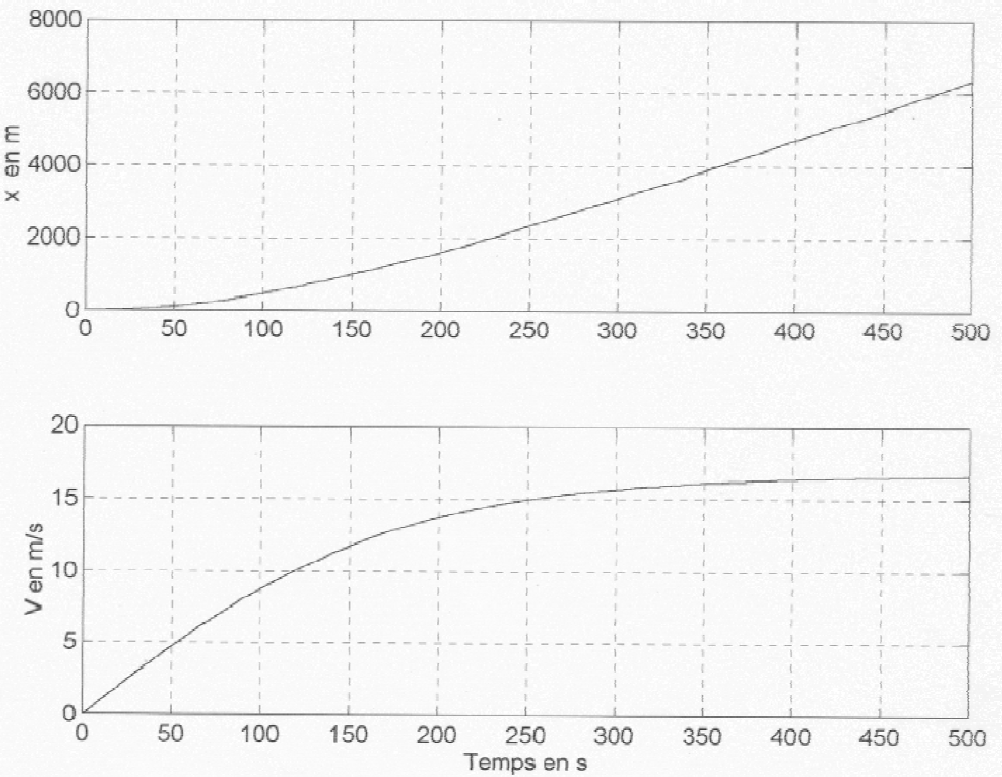
\includegraphics[width=\linewidth]{fig_04}
%\textit{}
\end{center}

\subsection*{Validation des performances statiques des motorisations}
On donne ci-dessous le schéma cinématique simplifié du mécanisme.

\begin{center}
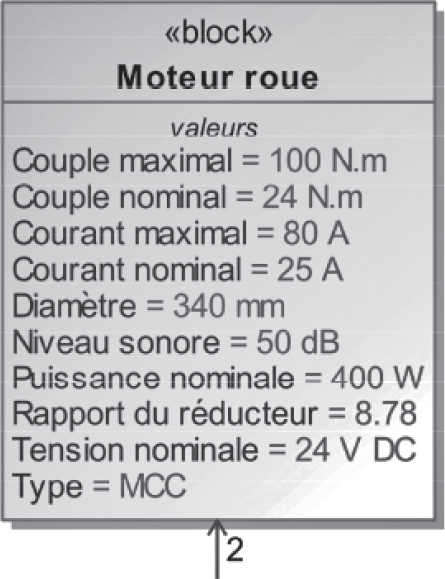
\includegraphics[width=\linewidth]{fig_02}
%\textit{}
\end{center}

Dans l’étude envisagée, les trois axes de rotation sont asservis en position angulaire et l’axe de translation de la pince \textbf{(4)} est asservi en effort. On va étudier le maintien en position réalisé par les trois axes de rotation. Dans cette phase, les trois moteurs maintiennent la position du robot le plus précisément possible et ce malgré les perturbations qu’engendrent les actions de pesanteur ainsi que les réactions dues aux efforts à l’extrémité de la pince \textbf{(4)}.

\noindent\textbf{Hypothèses}
\begin{itemize}
\item Étant données la très faible amplitude des mouvements et leur faible évolution dans le temps, une étude quasi statique est suffisante.
\item Le point $O_0 = O_{0,1,2,3}$ est supposé fixe.
\item Les actions mécaniques entre l’abdomen du patient et la pince \textbf{(4)} en $O_0$ seront négligées. On considère donc qu’il n’y a pas de liaison et d’action mécanique transmissible associée.
\item Les liaisons pivot et la liaison glissière sont toutes supposées parfaites (sans frottement).
\end{itemize}

\noindent\textbf{Modélisation des actions mécaniques}
\begin{itemize}
\item Le moteur \textbf{M1} et son réducteur, mettant en mouvement le solide \textbf{(1)} par rapport à \textbf{(0)}, permettent d’exercer en sortie de réducteur un couple sur \textbf{(1)} dont le moment est noté : $\vect{C}_{\text{m01}}=C_{\text{m01}}\vect{z_1}$.
%\item Le moteur \textbf{M2} et son réducteur, mettant en mouvement le solide \textbf{(2)} par rapport à \textbf{(1)}, permettent d’exercer en sortie de réducteur un couple sur \textbf{(2)} dont le moment est noté : $\vect{C}_{\text{m12}}=C_{\text{m12}}\vect{z_2}$.
%\item Le moteur \textbf{M3} et son réducteur, mettant en mouvement le solide \textbf{(3)} par rapport à \textbf{(2)}, permettent d’exercer en sortie de réducteur un couple sur \textbf{(3)} dont le moment est noté : $\vect{C}_{\text{m23}}=C_{\text{m23}}\vect{z_3}$.
\item De même, on note $\vect{C}_{\text{m12}}=C_{\text{m12}}\vect{z_2}$ et $\vect{C}_{\text{m23}}=C_{\text{m23}}\vect{z_3}$ les couples moteurs que \textbf{(1)} exerce sur \textbf{(2)} et \textbf{(2)} exerce sur \textbf{(3)}. 
%Le moteur \textbf{M3} et son réducteur, mettant en mouvement le solide \textbf{(3)} par rapport à \textbf{(2)}, permettent d’exercer en sortie de réducteur un couple sur \textbf{(3)} dont le moment est noté : $\vect{C}_{\text{m23}}=C_{\text{m23}}\vect{z_3}$.

\item On admettra que le moteur \textbf{M4} et son réducteur, mettant en mouvement la pince \textbf{(4)} par rapport à \textbf{(3)}, permettent d’exercer un glisseur en $O_4$ de résultante
$\vect{F}_{\text{m34}}=F_{\text{m34}}\vect{z_3}$.
\item L’action mécanique qu’exerce l’organe du patient sur la pince \textbf{(4)} est modélisable par un glisseur noté $\torseurstat{T}{\text{ext}}{4}=\torseurl{\vect{R}_{\text{ext}\to 4}=R_{\text{ext}\to 4}\vect{z_4}}{\vect{0}}{O_4}$ où $O_4$ est le point de contact entre \textbf{(4)} et l'organe du patient. 
\end{itemize}

\fi
\subsection*{Démarche globale}


\subparagraph{}
\textit{Réaliser le graphe d'analyse associé au système étudié.}
\ifprof
\begin{corrige}~\\

\begin{center} 
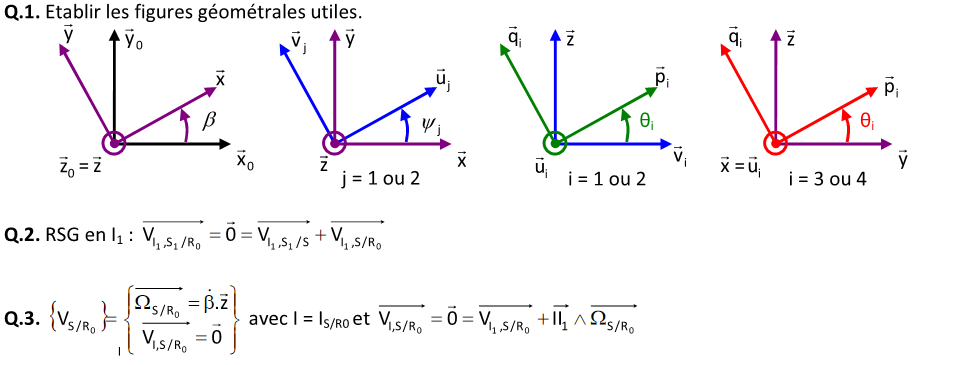
\includegraphics[width=\linewidth]{cor_01}
%\textit{}
\end{center}

\end{corrige}
\else
\fi
\subparagraph{}
\textit{Proposer la démarche (solide(s) isolé(s), théorème(s) utilisé(s)) permettant de déterminer les expressions littérales des couples $C_{\text{m01}}$, $C_{\text{m12}}$, $C_{\text{m23}}$,  et de la résultante $F_{\text{m34}}$,  lors de la phase de
maintien statique. Les calculs ne doivent pas être développés.}
\ifprof
\begin{corrige} ~\\

\begin{methode}
On cherche ici à déterminer le couple et les efforts à fournir par chacun des actionneurs pour maintenir en le système en équilibre statique. 4 actionneurs sont à déterminer, il faut donc un minimum de 4 équations. On va écrire les équations du PFS correspondant au mobilité afin de pas faire apparaître les inconnues de liaisons.   
\end{methode}

\begin{enumerate}
\item Pour déterminer $F_{\text{m34}}$ on isole le solide \textbf{(4)} et on applique le théorème de la résultante statique en projection sur $\vect{z_4}$.
\item Pour déterminer $C_{\text{m23}}$ on isole l'ensemble \textbf{(3+4)} et on applique le théorème du moment statique en $O$ en projection sur $\vect{z_3}$.
\item Pour déterminer $C_{\text{m12}}$ on isole l'ensemble \textbf{(2+3+4)} et on applique le théorème du moment statique en $O$ en projection sur $\vect{z_2}$.
\item Pour déterminer $C_{\text{m01}}$ on  isole l'ensemble \textbf{(1+2+3+4)} et on applique le théorème du moment statique en $O$ en projection sur $\vect{z_1}$.
\end{enumerate}
\end{corrige}
\else
\fi

 
 \subsection*{Modélisation simplifiée}
 
 \ifprof
 \else
\begin{itemize}
\item On se place dans une configuration particulière telle que 1 $\theta_1=45\degres$ et $\theta_2=\theta_3=0\degres$ ainsi que $O_4=O$. On donne pour cela les figures de calcul simplifiées.
\item Le centre d’inertie équivalent de l’ensemble matériel \textbf{E=(1+2+3+4)} est noté $G$.
Pour la configuration étudiée, la position de $G$ est considérée telle que $\vect{O_0G}=\ell\vect{z_2}$ . La masse totale de cet ensemble est notée $M=\SI{1,3}{kg}$. On prend $\ell=\SI{5}{cm}$. Le champ de pesanteur est noté $-g\vect{z_0}$ avec (avec $g=\SI{9,81}{m.s^{-2}}$).
\end{itemize}


\begin{center}
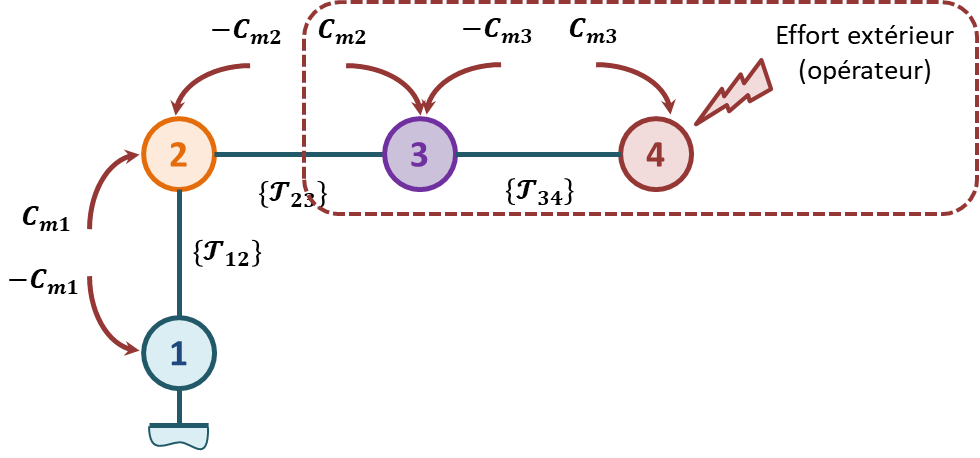
\includegraphics[width=\linewidth]{fig_05}
%\textit{}
\end{center}
\fi
\subparagraph{}
\textit{Déterminer analytiquement en fonction de $g$, $l$, $M$, $\theta_1$, $\alpha_1$ et $\alpha_2$, l'expression littérale de $C_{\text{m01}}$ lors de la phase de maintien statique. Effecteur l'application numérique (avec $\alpha_1=70\degres$ et $\alpha_2=-70\degres$).}
\ifprof
\begin{corrige} ~\\
\begin{itemize}
\item On isole l'ensemble \textbf{(1+2+3+4)}.
\item On réalise le bilan des actions mécaniques :
\begin{itemize}
\item action de la liaison pivot de 0 sur 1 : $\vectm{O}{0}{1}\vect{z_1}=0$.
\item action du moteur 0 sur 1 : $\vectm{O}{0_m}{1}\vect{z_1}=C_{\text{m01}}$.
\item action de la pesanteur sur $E$ :$\vectm{O}{\text{pes}}{E}\vect{z_1}$ : 
\begin{itemize}
\item $ \vectm{O}{\text{pes}}{E}\vect{z_1} = \underbrace{\vectm{G}{\text{pes}}{E}\vect{z_1}}_{\vect{0}}+\vect{OG}\wedge \left(-Mg\vect{z_0}\right)\cdot \vect{z_1}=-Mg\ell\left( \vect{z_2}\wedge\vect{z_0}\right)\cdot \vect{z_1}=-Mg\ell\left( \vect{z_0}\wedge\vect{z_1}\right)\cdot \vect{z_2}=-Mg\ell\sin\alpha_1\left( \vect{x_0}\cdot \vect{z_2} \right)=-Mg\ell\sin\alpha_1\left( \vect{x_0}\cdot \left(\cos\alpha_2\vect{z_1}-\sin\alpha_2\vect{y_1} \right) \right)=Mg\ell\sin\alpha_1\sin\alpha_2\cos\left( \dfrac{\pi}{2}+\theta_1\right)=Mg\ell\sin\alpha_1\sin\alpha_2\sin\theta_1$.
\end{itemize}
\item action de l'organe sur \textbf{(4)} : $\vectm{O}{\text{ext}}{4}\vect{z_1} =\vect{0}$.
\end{itemize}
\item On applique le théorème du moment statique en $O$ en projection sur $\vect{z_1}$ :
$$
C_m + Mg\ell\sin\alpha_1\sin\alpha_2\sin\theta_1 = 0.
$$
\end{itemize}

\item On réalise l'application numérique : $C_m=-Mg\ell\sin\alpha_1\sin\alpha_2\sin\theta_1 =-1,3\cdot 9,8 \cdot 0,05 \cdot \sin  70 \sin -70 \sin 45 = \SI{0,4}{Nm}$.
\end{corrige}
\else\fi

\subsection*{Retour sur la cahier des charges}

\subparagraph{}
\textit{En utilisant le diagramme de blocs et les résultats précédents, vérifier que l'exigence 1.1.1 peut être satisfaite. Remplir le diagramme suivant.}

\ifprof
\begin{corrige}
Le couple en sortie de réducteur est de $16\cdot 10^{-3} \cdot 66 = \SI{1,056}{Nm}$ ce qui est supérieur au couple nécessaire calculé à la question précédente. L'exigence 1.1.1 est donc validée .
\begin{center}
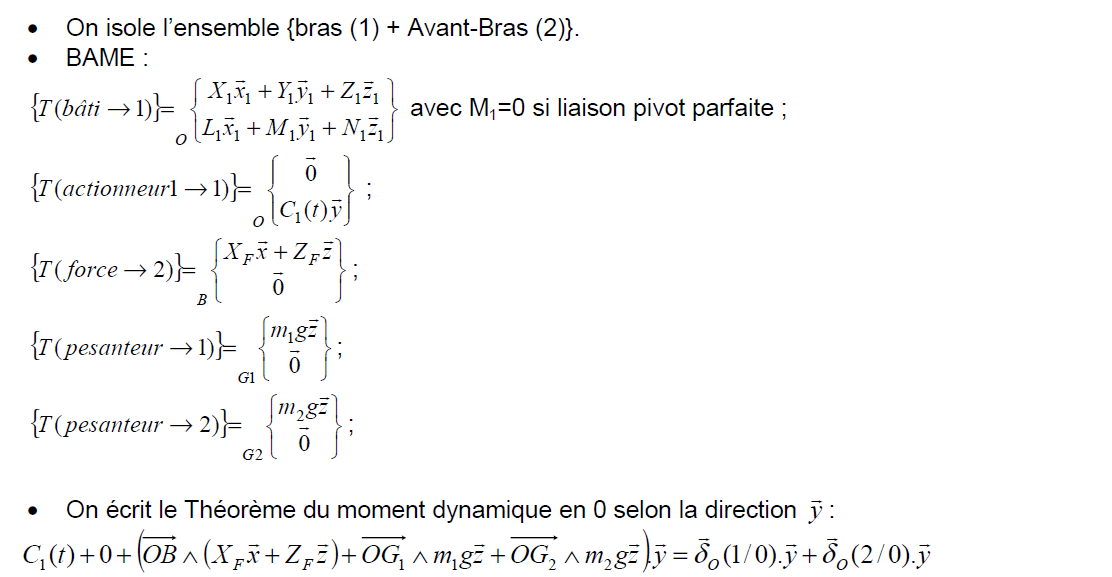
\includegraphics[width=.5\linewidth]{cor_02}
%\textit{}
\end{center}

\end{corrige}
\else
\fi

\ifprof
\else

\begin{center}
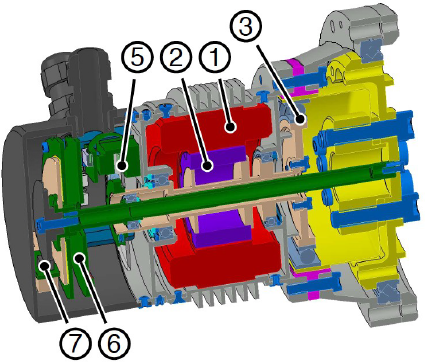
\includegraphics[width=\linewidth]{fig_06}
%\textit{}
\end{center}
\fi

\vspace{1cm}

\section*{Pour aller plus loin : Validation des performances de l'asservissement d'effort}
Lors du retrait de la vésicule, il est nécessaire de maintenir un effort constant en bout de pince \textbf{(4)}. Pour cela, on réalise un asservissement d'effort de l'axe en translation. 
\begin{obj}
Valider le positionnement du capteur d'effort et justifier la nécessité de faire une compensation de pesanteur. 
\end{obj}

\ifprof
\else
L'ensemble \textbf{(E)} contient ici la totalité de la transmission d’effort de la pince \textbf{(4)}, moteur M4 compris.
Dans cette partie, on simplifiera le modèle de contact entre abdomen et pince en retenant une liaison libre.
Pour deux configurations géométriques distinctes, le montage du capteur d’effort peut être modélisé par les
schémas cinématiques simplifiés ci-dessous.

\begin{center}
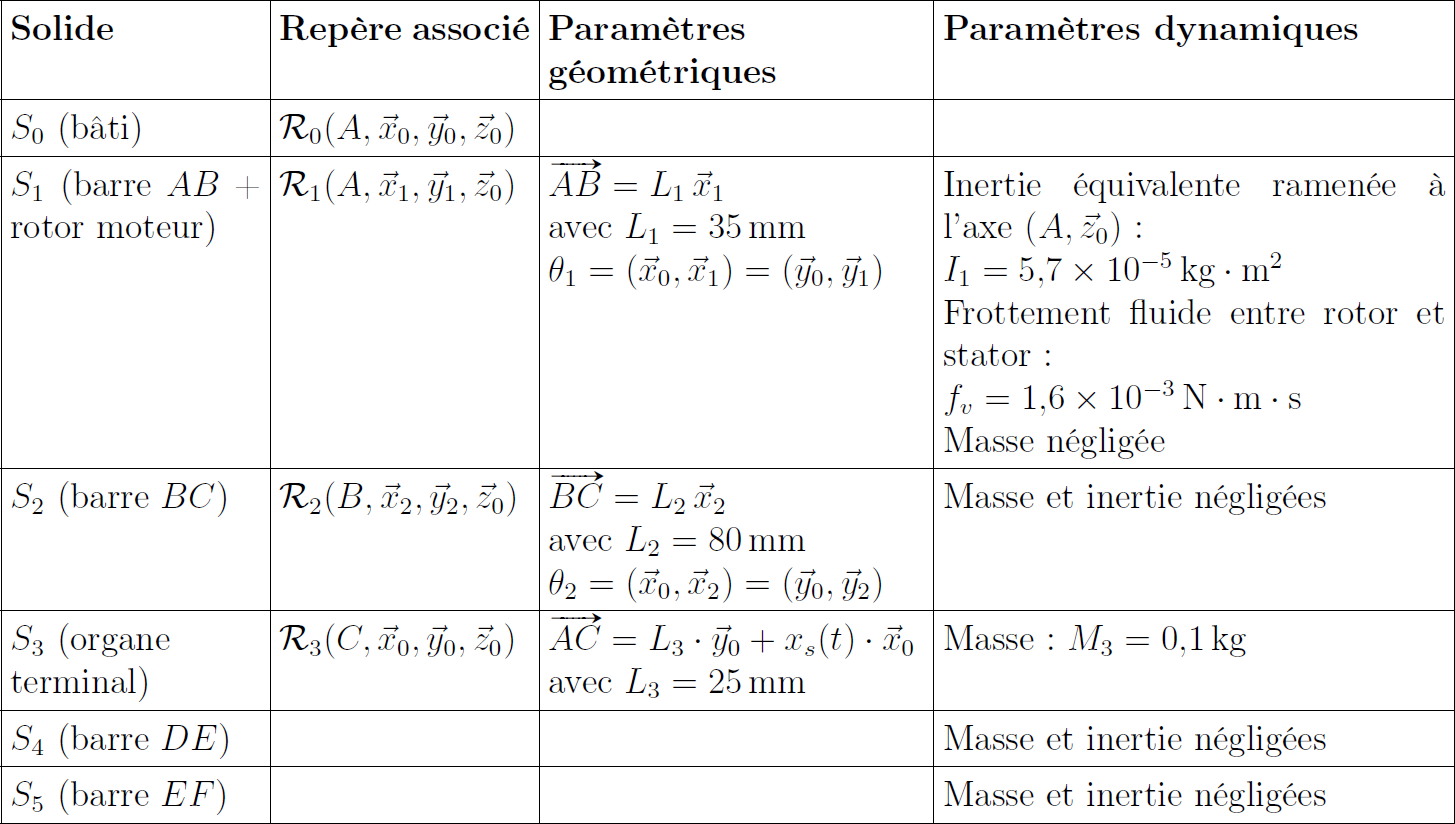
\includegraphics[width=\linewidth]{fig_07}
%\textit{}
\end{center}

Un ressort simulant la vésicule biliaire (raideur du ressort similaire à la
raideur de la vésicule) est installé en bout de pince.
\subsubsection*{Hypothèses}
\begin{itemize}
\item Le problème est plan.
\item Étant données les faibles vitesses et accélérations envisagées, une étude quasi-statique est
suffisante.
\item Les actions mécaniques de pesanteur sur \textbf{(E)} ne peuvent pas être négligées face aux actions mécaniques mises en jeu lors d’une opération. On notera leur résultante $\vect{P}_{(E)}$.
\item Le capteur d’effort assure la liaison entre l’ensemble \textbf{(0+1+2+3)} et \textbf{(E)}. Le capteur sera donc toujours en contact avec ces deux ensembles.
\end{itemize}
\subsubsection*{Modélisation des actions mécaniques}
\begin{itemize}
\item L'action mécanique qu’exerce le ressort sur l’ensemble \textbf{(E)} est modélisée par un glisseur noté $\torseurstat{T}{\text{Ressort}}{E}=\torseurl{\vectf{\text{Ressort}}{E}}{\vect{0}}{O_4}$ où $O_4$ est le point de contact entre la pince \textbf{(4)} et le ressort.
\item L'action mécanique, mesurée par le capteur, liée à sa liaison avec l'ensemble
\textbf{(E)}, est modélisée par
$\torseurstat{T}{\text{Capteur}}{E}=\torseurl{\vectf{\text{Capteur}}{E}}{\vectm{O_4}{\text{Capteur}}{E}}{O_4}$. La résultante sera notée $\vectf{\text{Capteur}}{E}=F_z\vect{z_3}+F_y\vect{y_3}$. Seules ces deux composantes seront prises en compte par la suite. 
\end{itemize}

Pour que la résultante de l’action mécanique mesurée par le capteur soit égale à la résultante de l’action mécanique que génère le ressort sur \textbf{(E)}, il faut
compenser la résultante de l’action mécanique de pesanteur.

\fi

\subparagraph{}
\textit{Pour la configuration 1 et par la méthode de votre choix, définir l’expression de $F_z$ et $F_y$ en fonction des autres actions mécaniques utiles. Commenter le résultat obtenu et la capacité du capteur à mesurer seulement les actions mécaniques générées par la pince sur le ressort.}

\ifprof
\begin{corrige}~\\

\begin{methode}
Dans la configuration 1, $\vect{z_0}=\vect{z_3}$ et $\vect{y_0}=\vect{y_3}$. On cherche des expressions suivant $\vect{z_0}$ et $\vect{y_0}$. Appliquer le théorème de la résultante statique suivant $\vect{y_0}$ et $\vect{z_0}$ devrait permettre de conclure. 
\end{methode}
\begin{itemize}
\item On isole \textbf{(E)}.
\item On réalise le bilan des actions mécaniques : 
\begin{itemize}
\item actions de pesanteur sur \textbf{(E)} de résultante $\vect{P}_{(E)}=-P\vect{z_0}$;
\item actions du ressort sur \textbf{(E)} de résultante $\vectf{\text{Ressort}}{E}=-F_{R\to E} \vect{z_0}$;
\item actions du capteur sur \textbf{(E)} de résultante $\vectf{\text{Capteur}}{E}=F_z\vect{z_0}+F_y\vect{y_0}$.
\end{itemize}
\item On applique le théorème de la résultante statique suivant $\vect{y_0}$ et $\vect{z_0}$ et on obtient : 
\begin{itemize}
\item $F_y = 0$. 
\item $F_z = P- F_{R\to E}$. 
\end{itemize}
\end{itemize}
Le capteur doit mesurer les actions de la pince sur le ressort. Or ici, l'effort va aussi dépendre du points de l’ensemble. Dans cette configuration, le capteur ne permet donc pas de dissocier l'effort de l'abdomen du poids du système.
\end{corrige}
\else
\fi

\ifprof
\else
La compensation de pesanteur revient à faire prendre en compte par le calculateur, en temps réel, la valeur des actions mécaniques de pesanteur quelle que soit la configuration géométrique du $\text{MC}^2\text{E}$. On pourra alors connaître, à partir de la mesure du capteur d’effort, l’action mécanique exercée par la pince \textbf{(4)} sur le ressort.

Pour comprendre le traitement de l’information que devra faire le calculateur on propose une deuxième configuration géométrique (configuration 2) du $\text{MC}^2\text{E}$.

\fi
\subparagraph{}
\textit{Dans la configuration 2, définir l’expression de $F_z$ et $F_y$ en fonction des autres actions mécaniques utiles. Pour réaliser la compensation, quels sont les paramètres à connaître en temps réel ?}
\ifprof
\begin{corrige} ~\\

\begin{methode}
Dans la configuration 2, appliquer le théorème de la résultante statique suivant $\vect{y_3}$ et $\vect{z_3}$ devrait permettre de conclure. 
\end{methode}
\begin{itemize}
\item On isole \textbf{(E)}.
\item On réalise le bilan des actions mécaniques : 
\begin{itemize}
\item actions de pesanteur sur \textbf{(E)} de résultante $\vect{P}_{(E)}=-P\vect{z_0}=-P\left(\cos\varphi  \vect{z_3}-\sin\varphi  \vect{y_3}\right)$;
\item actions du ressort sur \textbf{(E)} de résultante $\vectf{\text{Ressort}}{E}=-F_{R\to E} \vect{z_3}$;
\item actions du capteur sur \textbf{(E)} de résultante $\vectf{\text{Capteur}}{E}=F_z\vect{z_3}+F_y\vect{y_3}$.
\end{itemize}
\item On applique le théorème de la résultante statique suivant $\vect{y_3}$ et $\vect{z_3}$ et on obtient : 
\begin{itemize}
\item $F_y = -P\sin\varphi $. 
\item $F_z = P\cos\varphi  - F_{R\to E}$. 
\end{itemize}
\end{itemize}
Si $\varphi$ est une valeur connue, la mesure suivant $\vect{y_3}$ permet de déterminer le poids de l'ensemble. Connaissant $P$, la mesure suivant $\vect{z_3}$ permet alors de déterminer l'action mécanique du ressort. 
\end{corrige}
\else
\fi



\subsection*{Retour sur le cahier des charges}
\ifprof
\else


Le montage d’essai suivant a été mis en place. La seconde configuration a été réalisée avec un angle $\varphi$ de 20\degres. Cet essai, réalisé sans interaction entre le ressort et la pince \textbf{(4)}, a permis d’obtenir les valeurs expérimentales suivantes mesurées par le
capteur.
\begin{center}
\begin{tabular}{|c|c|c|c|}
\hline
\multicolumn{2}{|c|}{Configuration 1}&\multicolumn{2}{c|}{Configuration 2}\\ \hline
$|F_{y0}|$ & $|F_{z0}|$ & $|F_{y20}|$ & $|F_{z20}|$ \\ \hline
\SI{0,0222}{N} & \SI{12,753}{N} & \SI{4,382}{N} & \SI{11,999}{N} \\ \hline
\end{tabular}
\end{center}

\fi
\subparagraph{}
\textit{Estimer la valeur du poids. Donner une estimation de la fiabilité sur la détermination du poids par les capteurs d'efforts. 
Pour réaliser la compensation de pesanteur, comment doivent être utilisées ces grandeurs mesurées ?}
\ifprof
\begin{corrige} ~\\
On ne connaît pas le poids de l'ensemble qui devrait être une donnée. On va donc le déduire du montage expérimental. En utilisant les expressions de la question précédente, on déduit que $P\simeq  \SI{12,753}{N}$ . 

Dans la seconde configuration, on a $|P|=\dfrac{|F_{y20}|}{\sin\varphi}=\dfrac{4,382}{\sin 20}\simeq \SI{12,81}{N}$ ou  $|P|=\dfrac{|F_{z20}|}{\cos\varphi}=\dfrac{11,999}{\cos 20}\simeq \SI{12,77}{N}$.

Ainsi, une estimation de l'erreur peut être donnée par : $e=\dfrac{12,81-12,753}{12,753}\simeq0,4\%$

\begin{center}
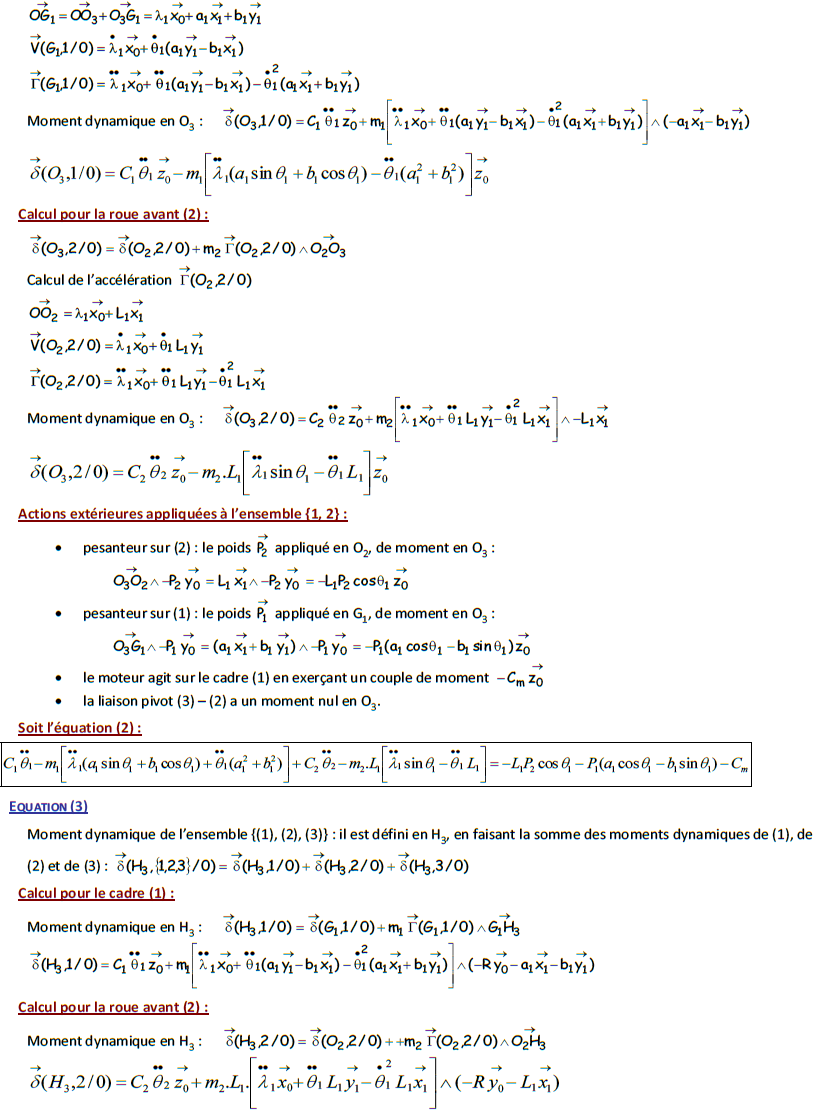
\includegraphics[width=\linewidth]{cor_03}
%\textit{}
\end{center}

%
%\begin{center}
%\begin{tabular}{l|c|c|c|c|}
%\cline{2-5}
%&\multicolumn{2}{|c|}{Configuration 1}&\multicolumn{2}{c|}{Configuration 2}\\ \cline{2-5}
%&$|F_y|$ & $|F_z|$ & $|F_y|$ & $|F_z|$ \\ \cline{2-5}
%Expérimental &\SI{0,0222}{N} & \SI{12,753}{N} & \SI{4,382}{N} & \SI{11,999}{N} \\ \cline{2-5}
%Théorique &\SI{0}{N} & \SI{12,753}{N} & \SI{4,382}{N} & \SI{11,999}{N} \\ \cline{2-5}
%\end{tabular}
%\end{center}


\end{corrige}
\else
\begin{center}
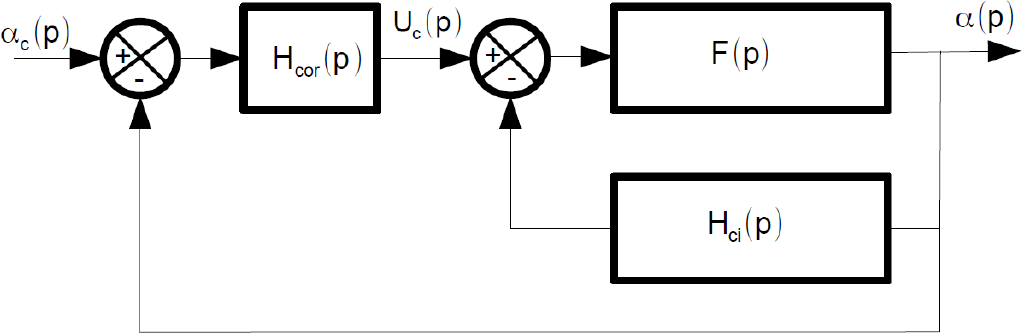
\includegraphics[width=\linewidth]{fig_08}
%\textit{}
\end{center}

\fi



\ifprof
\else
\begin{center}
\begin{tabular}{|p{.95\linewidth}|}
\hline
\textbf{Corrigé résumé}
\begin{enumerate}
\item $\quad$
\item $\quad$
\item $C_m=-Mg\ell\sin\alpha_1\sin\alpha_2\sin\theta_1 =\SI{0,4}{Nm}$.
\item $\quad$
\end{enumerate} \\
\hline
\end{tabular}
\end{center}
\fi
\ifprof
\else
\end{multicols}
\fi

\ifprof
\else

\vspace{1cm}
\begin{center}
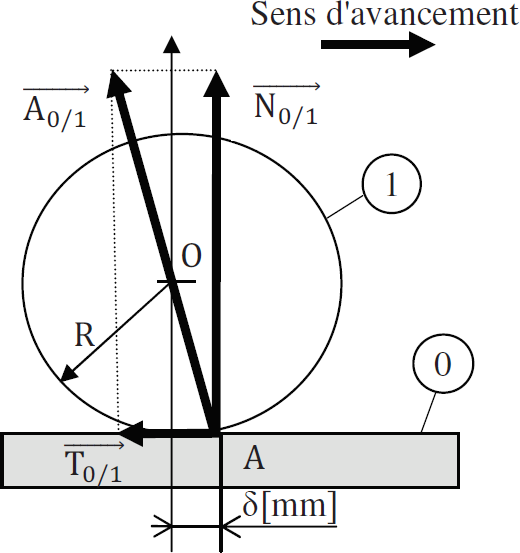
\includegraphics[width=\linewidth]{fig_03}
%\textit{}
\end{center}
\fi
